% This is an example of how to format a thesis with LaTeX the
% simplest possible way (permitted beginning in 2010).
% NO UGA STYLE SHEET IS NEEDED.

\documentclass[12pt]{report}
\usepackage{fullpage}
\usepackage{setspace}\doublespacing    % important!
\usepackage{graphicx}
\usepackage{cite}
\usepackage{adjustbox}
\textfloatsep 0.75in                   % important with double spacing

\begin{document}

% Make the official abstract page
\newpage
\thispagestyle{empty}
\vspace*{18pt}
\begin{center}
\textsc{Structure Forming Processes in\\Mesoscopic Polymer Systems}\\[18pt]
by\\[18pt]
\textsc{Tomas Koci}\\[12pt]
(Under the direction of Michael Bachmann)\\[12pt]
\textsc{Abstract}
\end{center}
This is going to be the best abstract ever :)

% Display the index words (this is a bit fancy):
\begin{list}{\sc Index words:\hfill}{\labelwidth 1.2in\leftmargin 1.4in\labelsep 0.2in}
\item 
\begin{flushleft}\singlespacing
Polymer Aggregation,
Monte Carlo Simulations,
Parallel Tempering,
Multicanonical Sampling,
Canonical Analysis, 
Microcanonical Inflection-Point Analysis,
Flexible Polymer,
Structural Transitions,
Finite Systems,
Finite-Size Effects
\end{flushleft}
\end{list}



% Make the official title page
\newpage
\thispagestyle{empty}
\vspace*{18pt}
\begin{center}
\textsc{Structure Forming Processes in\\Mesoscopic Polymer Systems}\\[18pt]
by\\[18pt]
\textsc{Tomas Koci}\\[12pt]
B.A., The Juilliard School, 2008\\
\vfill
A Dissertation Submitted to the Graduate Faculty \\
of The University of Georgia in Partial Fulfillment \\
of the \\
Requirements for the Degree \\[10pt]
\textsc{Doctor of Philosophy}\\[36pt]
\textsc{Athens, Georgia}\\[18pt]
2016
\end{center}

% Make the copyright page
\newpage
\thispagestyle{empty}
\vspace*{5.5in}
\begin{center}
\copyright 2016 \\
Tomas Koci \\
All Rights Reserved
\end{center}

% Make the approval page
\newpage
\thispagestyle{empty}
\vspace*{18pt}
\begin{center}
\textsc{Structure Forming Processes in\\Mesoscopic Polymer Systems}\\[18pt]
by\\[18pt]
\textsc{Tomas Koci}
\end{center}
\vfill
\begin{flushleft}\singlespacing
\hskip 200pt {Approved:}\\
\vskip 12pt
% Two major professors.  If you have only one, change word to "Professor".
\hspace*{200pt}\makebox[100pt][l]{Major Professor:}Michael Bachmann\\
\vskip 12pt
% Committee (use as many lines as needed)
\hspace*{200pt}\makebox[100pt][l]{Committee:       }Steven P. Lewis\\
\hspace*{200pt}\makebox[100pt][l]{~                }Heinz-Bernd Schuttler\\
% Approval words
\vfill
Electronic Version Approved:\\[12pt]
Alan Dorsey\\
Dean of the Graduate School\\
The University of Georgia\\
July 2016
\end{flushleft}


% Now we begin the regular LaTeX document.
% You may want to have a regular LaTeX title page here...

\chapter*{Acknowledgments}
\addcontentsline{toc}{chapter}{Acknowledgments}
\pagenumbering{roman}
\setcounter{page}{4}

\setcounter{tocdepth}{1}
\tableofcontents
\listoffigures  % if any
\addcontentsline{toc}{chapter}{\listfigurename}
\listoftables % if any
\addcontentsline{toc}{chapter}{\listtablename}
\chapter{Introduction}
\pagenumbering{arabic}
\setcounter{page}{1}
Kickass intro...


\chapter{Elements of Statistical Mechanics}
\label{chap:elements_of_stat_mech}
Statistical mechanics aims at explaining the microscopic origins of macroscopic properties of systems with large numbers of degrees of freedom. The exact solution for the time evolution of every particle in a single complex system requires enormous computational efforts, and in most cases provides little insight. In contrast to the chaotic motion of particles at the microscopic level, collective system properties such as entropy, pressure, or temperature, for the most part exhibit relatively simple behavior. The formalism of statistical mechanics allows us to study these properties by considering the average behavior of a large number of identically prepared systems, i.e., the statistical ensemble. It is well established, that for very large systems near the thermodynamic limit, all ensembles become equivalent. However this is emphatically not true in the case of intrinsically finite systems for which the choice of an ensemble is non-trivial\cite{Bachmann2014}. Therefore, I shall briefly discuss several prominent statistical ensembles, starting with arguably the most fundamental one, the \textit{microcanonical ensemble}.

\section{The microcanonical ensemble}
\label{sec:mic_ensemble}
Let us consider a mechanically and adiabatically isolated system with a constant number of particles $(N)$, volume $(V)$, and energy $(E)$. At any given moment, the system is to be found in a particular microstate $\mu$, which is represented by a point in a $6N$ dimensional phase-space. At a fixed energy $E$, the accessible microstates are constrained to the surface of constant energy $\mathcal{H}(\mu) = E$, where $\mathcal{H}$ is the Hamiltonian of the system. The total number of microstates corresponding to a macrostate with a fixed energy $E$ is obtained by calculating the density of states\footnote{Please refer to section 2.3 for detailed discussion of alternative definitions of the density of states.}
\begin{equation}
\label{eq:densityOfStatesTheoretic}
g(E) = \int \mathcal{DP}\mathcal{DQ} \:\: \delta(E - \mathcal{H}(\mathcal{P},\mathcal{Q})),
\end{equation} 
where 
\begin{equation}
\mathcal{DP}\mathcal{DX} = \prod_{n = 1}^{N} \frac{d^{3}p_{n}d^{3}x_{n}}{(2 \pi \hbar)^{3}}
\end{equation}
is the Lebesgue measure over phase space\cite{Rugh2001}. In computational studies, the energy space is by necessity discretized into intervals of width $\Delta E$, and the density of states $g(E_{i})$ is obtained by counting the microstates within a thin shell of width $\Delta E$. Formally, $g(E_{i})$ is a discrete function defined as
\begin{equation}
\label{eq:densitOfStatesExplicit}
g(E_{i}) = \int _{E_{i}-\Delta E/2} ^{E_{i}+\Delta E/2} g(E)dE,
\end{equation}
where $g(E)$ in the integrand is the continuous density of states\cite{Bachmann2014}.

Assuming that no additional quantities are conserved, i.e. the system is ergodic, all accessible microstates have equal a priori probabilities\cite{Kardar2007}. The microcanonical equilibrium probability distribution is given by 
\begin{equation}
p(\mu)_{E} = \left\{
\begin{array}{lr}
1/g(E), & \quad
\mathrm{if} \: \mathcal{H(\mu)} = E\\
0, & \quad \mathrm{if} \: \mathcal{H(\mu)} \neq E,
\end{array}
\right.
\end{equation}
and the expectation value of an observable $O$ at a fixed energy $E$ is found by averaging over the surface of constant energy
\begin{equation}
\left< O \right>_{E} = \int \mathcal{DP}\mathcal{DQ} \:\: O(\mathcal{P},\mathcal{Q}) \:\: \delta(E - \mathcal{H}(\mathcal{P},\mathcal{Q})).
\end{equation}
The density of states of a typical mesoscopic system can easily span several thousands of orders of magnitude. It is therefore convenient to define the microcanonical equilibrium entropy
\begin{equation}
S(E) = k_\mathrm{B}\, \mathrm{ln}\, g(E),
\end{equation}
as an \textit{extensive} quantity with dimensions of energy over temperature.\footnote{If temperature is measured in the more natural units of energy, entropy becomes a unitless quantity and the Boltzmann constant equals to unity.}


\subsection{Microcanonical temperature}
Temperature is one of the most fundamental concepts of statistical mechanics. Traditionally, it has been defined in terms of average kinetic energies of particles in a system\cite{Pathria}. In the following, we wish to motivate a more fundamental definition and introduce temperature as an intrinsic system property which can be obtained directly from the microcanonical density of states. For this purpose, let us consider an adiabatically isolated system composed of two weakly interacting subsystems, $S_{1}$ and $S_{2}$. The energy of the combined system is constant and can be written as the sum of the energies of the two subsystems $E = E_{1} + E_{2}$. At a fixed system energy $E$, the probability density for subsystem $S_{1}$ to contain energy $E_{1}$ is written as 
\begin{equation}
\rho(E_{1})_{E} = \frac{g_{1}(E_{1})g_{2}(E-E_{1})}{g(E)}.
\end{equation}
The density of states of the combined system is given by the convolution of the subsystem densities
\begin{equation}
\label{eq:DOSConvolution}
g(E) = \int dE_{1}g_{1}(E_{1})g_{2}(E-E_{1}).
\end{equation}
In systems with many degrees of freedom, the probability density $\rho(E_{1})_{E}$ is a sharply peaked distribution around the equilibrium energy $\bar{E}_{1}$\footnote{The energy fluctuations per particle around the equilibrium energy $\bar{E}_{1}$ scale as $N^{-1/2}$\cite{Sethna2006}.}. Hence the convolution in Eq. \ref{eq:DOSConvolution} can be well approximated by the maximum value of the integrand\cite{Sethna2006}. The maximum is found when the derivative of the integrand with respect to $E_{1}$ is set to zero. It follows that
\begin{equation}
\frac{1}{g_{1}}\frac{dg_{1}}{dE_{1}}\bigg|_{\bar{E}_{1}} = \frac{1}{g_{2}}\frac{dg_{2}}{dE_{2}}\bigg|_{E - \bar{E}_{1}},
\end{equation}
or alternatively in terms of the microcanonical entropy
\begin{equation}
\frac{dS_{1}}{dE_1}\bigg|_{\bar{E}_{1}} = \frac{dS_{2}}{dE_{2}}\bigg|_{E - \bar{E}_{1}}.
\end{equation}
In analogy to the familiar observation that interacting systems at thermal equilibrium have equal temperatures, we define the microcanonical temperature as 
\begin{equation}
T(E) = \left(\frac{dS(E)}{dE}\right)^{-1}.
\end{equation}
Frequently, it is more convenient to consider instead the inverse microcanonical temperature 
\begin{equation}
\beta(E) = \frac{dS(E)}{dE}.
\end{equation}

\subsection{Microcanonical analysis of phase transitions}
\label{subsec: micro_analysis}
A macrostate of a system is specified by a set of macroscopic variables and possesses the characteristics of the predominant microstates. Macrostates are said to belong to the same thermodynamic phase, if in a given range of some external control parameters\footnote{Some common examples of external control parameters are the canonical temperature, pressure, or the chemical potential.} all of the system's thermodynamic observables are analytic, i.e. have convergent Taylor expansions. Singularities in the observables signify the presence of phase transitions between distinct phases, typically marked by abrupt changes in macrosopic properties in response to minute variations of external control parameters. Phase transitions can be roughly divided into two categories. \textit{Abrupt} transitions are characterized by the coexistence of two distinct phases and discontinuities in most physical properties. \textit{Continuous} transitions, although less common in nature, have been the object of most intense research. They are marked by diverging correlation lenghts, large fluctuations, and scale invariance\cite{Sethna2006}. 

Divergences and singularities in thermodynamic observables and their derivatives are only found in systems which satisfy the thermodynamic limit. In mesoscopic systems\footnote{Typical length scales in  mesoscopic systems are of the order of $\sim 10  10^{3}$ nanometers. In this regime, exact quantum many-body interactions can be replaced by effective classical potentials, and cooperative effects dominate structure formation processes. Mesoscopic systems are distinct from macroscopic systems due to the presence of significant finite-size effects, which disallow the simplifying assumptions of the thermodynamic limit.}, due to finite size effects, divergences are replaced by peaks and discontinuities are smoothed over\cite{Bachmann2014}. For clarity, we designate the term \textit{pseudophase transition} to represent significant conformational changes in finite systems. Likewise, thermodynamic phases in finite systems shall be referred to as \textit{pseudophases}. In the following, we present a powerful formalism for the analysis of pseudophase transitions in the microcanonical ensemble; the microcanonical inflection point analysis.

\subsubsection{Microcanonical inflection-point analysis}
Unlike its canonical counterpart~-- the heat-bath temperature~-- the
microcanonical inverse temperature is an inherent property of the system, derived directly from the fundamental microcanonical quantities $S(E)$ and $E$. We assert that all essential information about energetically and entropically driven thermodynamic processes is contained in its curvature. Hence the microcanonical inverse temperature is an ideal starting point for a comprehensive analysis of pseudophase transitions\cite{Gross2001}.  

%
\begin{figure}
\center
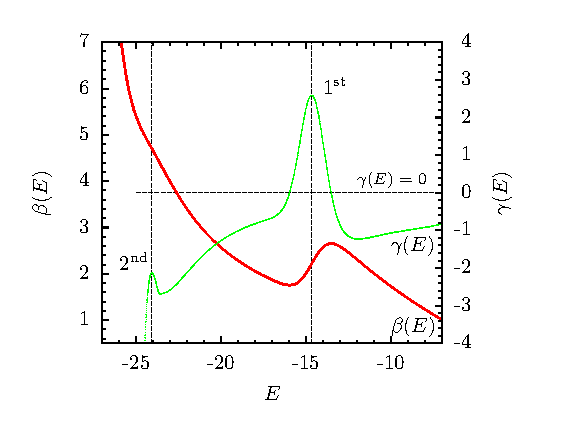
\includegraphics[width = 0.7\textwidth]{chapter2Figs/MicroAnalysisExample.eps}
\caption{\label{fig:Fig_1}%
Microcanonical inflection-point analysis of the inverse microcanonical temperature $\beta(E)$. The prominent back-bending region in $\beta(E)$, together with the positive-valued peak in its energy derivative $\gamma(E)$ at $E \approx -15$, indicates a first-order transition. The negative-valued peak at $E\approx -24$ corresponds to a second-order transition.}
\end{figure}
%

In analogy to the principle of minimal sensitivity~\cite{Stevenson}, structural transitions between pseudophases occur when $\beta(E)$, or one of its energy
derivatives, respond least sensitively to variations in energy\cite{Schnabel2011}. In particular, first-order transitions are associated with inflection points in $\beta (E)$ that have a positive slope, accompanied by positive-valued peaks in the energy derivative $\gamma(E)=d\beta(E)/dE$. Similarly, a second-order transition occurs when $\beta(E)$ exhibits an inflection point with a negative slope and $\gamma(E)$ attains a negative-valued peak. Examples of microcanonical pseudophase transition signals are shown in Fig.~\ref{fig:Fig_1}. The formalism can be naturally extended to higher-order transitions. Inflection point in the $(2\mathrm{n})$th-derivative of entropy, accompanied by a positive-valued valley in the $(2\mathrm{n}+1)$th-derivative, indicates a $(2\mathrm{n}+1)$th-order transition. Similarly, a $(2\mathrm{n})$th-order transition is marked by an inflection point in the $(2\mathrm{n}-1)$th-derivative of entropy and a negative-valued peak in the $(2\mathrm{n})$th-order derivative.

%
\begin{figure}
\center
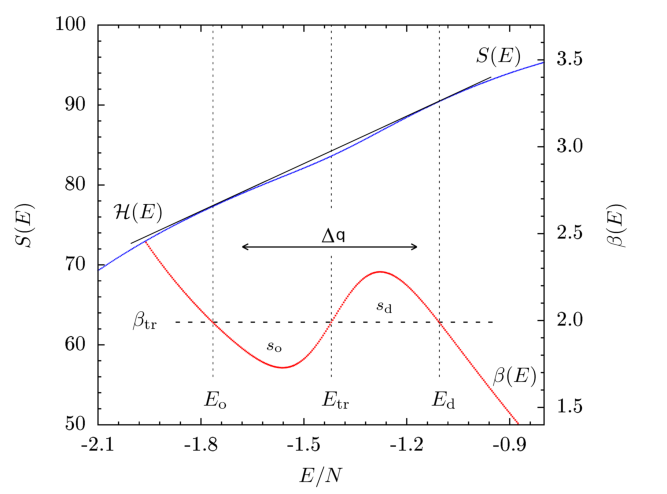
\includegraphics[width = 0.7\textwidth]{chapter2Figs/maxwellConstruct.pdf}
\caption{\label{fig:Fig_2}%
The convex region of the microcanonical entropy $S(E)$ and the back-bending of the microcanonical inverse temperature $\beta(E)$ are prominent indicators of \textit{first-order} transitions. The slope of the double-tangent Gibbs hull $\mathcal{H}(E)$ defines the transition temperature $\beta_{\mathrm{tr}}$. The Maxwell construction, defined by equal areas of $s_{\mathrm{o}}$ and $s_{\mathrm{d}}$, is itself positioned at $\beta_{\mathrm{tr}}$. The transition energy $E_{\mathrm{tr}}$ indicates the location of the largest separation between $\mathcal{H}(E)$ and $S(E)$, which signifies maximal entropic suppression of the transition states. The latent heat $\Delta Q$ corresponds to the width of the transition region between $E_{\mathrm{d}}$ and $E_{\mathrm{o}}$.}
\end{figure}
%
Alternatively, in the case of first-order transitions, the transition temperature $\beta_{\mathrm{tr}}$ can be obtained by the means of the Maxwell construction which was originally introduced to repair the unphysical back-bending in the pressure versus volume isotherms for the van der Waals gas. In mesoscopic systems, the finite-size effects lead to the entropic suppression of transition states, which is manifested in the backbending of $\beta(E)$ and the convex intruder in $S(E)$. The position of the Maxwell construction is determined by the equality of the areas $s_{\mathrm{o}}$ and $s_{\mathrm{d}}$ [Fig.\ref{fig:Fig_2}]. Commonly referred to as \textit{surface entropies}, $s_{\mathrm{o}}$ and $s_{\mathrm{d}}$ are defined as the integrals
\begin{eqnarray}
\label{eq:surfaceEntr}
s_{\mathrm{o}} &=& \int_{E_{\mathrm{o}}}^{E_{\mathrm{tr}}} dE \:\: (\beta_{\mathrm{tr}}-\beta(E)), \\
s_{\mathrm{d}} &=& \int_{E_{\mathrm{tr}}}^{E_{\mathrm{d}}} dE \:\: (\beta(E)-\beta_{\mathrm{tr}}).
\end{eqnarray}
The Maxwell line intersects the inverse temperature at the energies $E_{\mathrm{o}}$, $E_{\mathrm{tr}}$, and $E_{\mathrm{d}}$. The latent heat
$\Delta Q = E_{\mathrm{d}} - E_{\mathrm{o}}$ corresponds to the energetic separation between the ordered and the disordered pseudophases . The transition energy $E_{\mathrm{tr}}$ indicates the location where intermediate states experience the maximal entropic suppression\cite{Bachmann2014}.

The slope of the double-tangent Gibbs construction, also shown in Figure \ref{fig:Fig_2}, provides yet another definition of $\beta_{\mathrm{tr}}$. As a function of energy, the Gibbs hull is defined as
\begin{equation}
\mathcal{H}(E) = S(E_{\mathrm{o}}) + \beta_{\mathrm{tr}}[E-E_{\mathrm{o}}],
\end{equation}
where $\beta_{\mathrm{tr}}$ can be expressed in terms of the energy and entropy differences between the ordered and disordered pseudophases as
\begin{equation}
\beta_{\mathrm{tr}} = \frac{S_{\mathrm{d}}-S_{\mathrm{o}}}{E_{\mathrm{d}}-E_{\mathrm{o}}} = \frac{\Delta S}{\Delta Q}.
\end{equation}
With the exception of composite multi-step transitions, characterized by additional oscillations in the back-bending region of $\beta(E)$, the transition temperatures obtained by the means of the Maxwell and Gibbs constructions are identical.

The formalism of the microcanonical inflection-point analysis makes no reference to the thermodynamic limit. In fact, it is equally suitable for analysis of macroscopic and mesoscopic systems alike. This is in stark contrast to the more traditional canonical analysis which is defined under the assumption of the thermodynamic limit and has to be modified for the treatment of finite systems.

 
 
\section{The canonical ensemble}
\label{sec:canonicalEnsemble}
The canonical ensemble describes the behavior of a closed system which is in thermal equilibrium with a large external heat bath at a fixed temperature $T$. In analogy to the density of states in the microcanonical ensemble, the partition function $Z(T)$ contains all the essential information about the thermodynamic properties of the system under consideration\cite{Landau2000}. It can be defined directly as a Laplace transform\footnote{Here we assume that the system under investigation has discrete energy levels, which is always true in the context of computational studies. In the case of a continuous energy spectrum, the discrete sum is replaced by the integral $Z(T) = \int dE \:\:  g(E) e^{-\frac{E}{k_{\mathrm{B}}T}}$.} of the microcanical density of states $g(E)$
\begin{equation}
Z(T) = \sum_{i} g(E_{i}) e^{-\frac{E_{i}}{k_{\mathrm{B}}T}},
\end{equation}
where $T$ is the canonical temperature and $k_{\mathrm{B}}$ is the Boltzmann constant. The condition of thermal equilibrium prohibits any net average energy transfer between the system and the heat bath. However, the system can temporarily gain or loose energy through constant fluctuations and dissipations. The probability for a given microstate $\mu$ at a temperature $T$ is given by the Boltzmann distribution
\begin{equation}
p(\mu) = \frac{1}{Z(T)}e^{-\frac{\mathcal{H}(\mu)}{k_{\mathrm{B}}T}},
\end{equation}
where $\mathcal{H}$ is the Hamiltonian of the system. The appropriate thermodynamic potential in the canonical ensemble is the Helmholtz free energy
\begin{equation}
F(T) = -k_{\mathrm{B}}T \: \mathrm{ln}\, Z(T).
\end{equation}
This quantity represents the energy available to perform work and can be used to obtain all other thermodynamic quantities by differentiation\cite{Pathria,Sethna2006}. The temperature derivative of the free energy defines the canonical entropy
\begin{equation}
\label{eq:canonicalEntropy}
S(T) = -\frac{\partial}{\partial T}F(T)\bigg|_{N,V},
\end{equation} 
which measures the amount of disorder in the system.
The internal energy $U$, defined as a sum over all microstate energies weighted by the Boltzmann distribution  
\begin{equation}
\label{eq:InternalEnergy}
U(T) = \frac{\sum_{\mu} \mathcal{H}(\mu)e^{-\frac{\mathcal{H}(\mu)}{k_{\mathrm{B}}T}}}{Z(T)} =  \frac{\sum_{E} E \, g(E) e^{-\frac{E}{k_{\mathrm{B}}T}}}{Z(T)},
\end{equation}
represents the average energy of the system. Alternatively, the internal energy can be obtained by the differentiation of the free energy
\begin{equation}
U(T) = k_{\mathrm{B}}T^{2}\frac{\partial}{\partial T} \mathrm{ln} Z(T)\bigg|_{N,V}
= -T^{2}\frac{\partial}{\partial T}\left(\frac{F}{T}\right)\bigg|_{N,V}.
\end{equation}
\newpage
\noindent
The amount of energy needed to increase the temperature of the system by one unit is given by the specific heat 
$C_{V}$, defined as a temperature derivative of the internal energy
\begin{equation}\label{eq:22}
C_{V}(T) = \frac{\partial}{dT}U(T)\bigg|_{N,V} = -T\frac{\partial^{2}}{\partial T^{2}}F(T)\bigg|_{N,V}.
\end{equation}
On the other hand, starting with the third term in equation \ref{eq:InternalEnergy} we obtain the following expression 
\begin{eqnarray}
C_{V}(T) &=&  \frac{\partial}{dT}\frac{\sum_{E} E \, g(E) e^{-\frac{E}{k_{\mathrm{B}}T}}}{Z(T)} = -\frac{1}{k_{\mathrm{B}}T^2}\frac{\partial}{\partial \beta}\frac{\sum_{E} E \, g(E) e^{-\beta E}}{\sum_{E}g(E) e^{-\beta E}} \nonumber \\
&=& \frac{1}{k_{\mathrm{B}}T^2} \left[\left(\frac{\sum_{E} E^{2} \, g(E)  e^{-\beta E}}{Z(T)}\right) - \left(\frac{\sum_{E} E \, g(E)  e^{-\beta E}}{Z(T)}\right)^{2}\right] \nonumber \\
&=& \frac{1}{k_{\mathrm{B}}T^2}\left(\left<E^{2}\right> - \left<E\right>^{2}\right),
\end{eqnarray}
where the last expression corresponds to the variance of the Boltzmann distribution. This result is of a profound physical importance, establishing the connection between the macroscopic response quantity $C_{V}$, and microscopic fluctuations.

\subsection{Canonical analysis of phase transitions}
Sudden dramatic changes of macroscopic properties, in response to small variations of an external control parameter, indicate that the system under investigation is undergoing a phase transition. Here we consider temperature-driven transitions and describe a classification scheme similar to Ehrenfest's.

In the thermodynamic limit, it is generally possible to identify some property of the system which is non-zero in the ordered phase and zero in the disordered phase, i.e. the order parameter\cite{Bachmann2014,Landau2000}. A standard example is the magnetization $m$ in a ferromagnetic system, where $m = 1$ in the ordered ferromagnetic phase and $m = 0$ in the disordered paramagnetic phase. The derivative of the order parameter with respect to its conjugate variable defines a response quantity\footnote{In the case of the magnetization $m$, the appropriate conjugate thermodynamic variable is the external field $H$, and the corresponding response quantity is the magnetic susceptibility $\chi$.} which is discontinuous at the transition point. Order parameters also play a central role in the formulation of the Landau theory, where they serve as a basis for the expansion of the free energy around the transition point\cite{Kardar2009}. 

\begin{figure}
\center
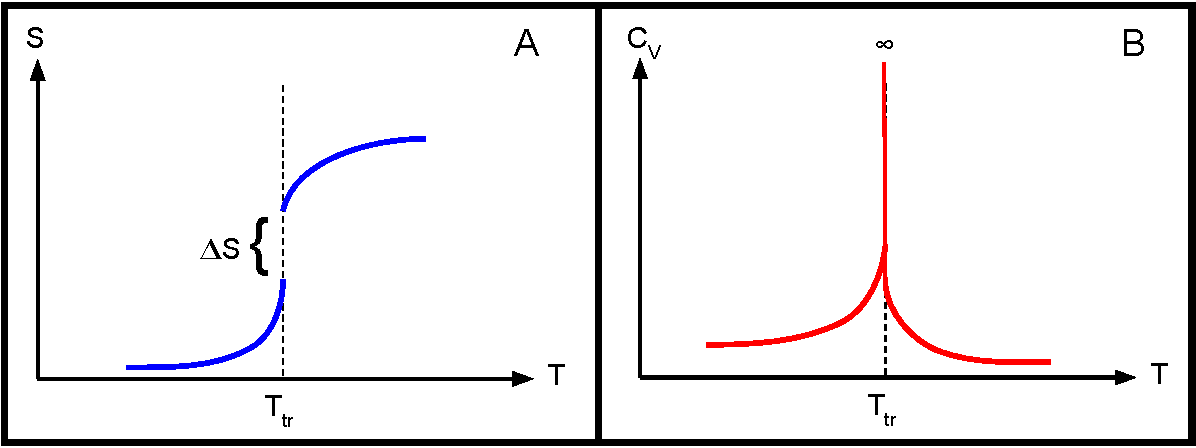
\includegraphics[width = 0.8\textwidth]{chapter2Figs/CanonicalFirstOrder.pdf}
\caption{\label{fig:Fig_3}% 
(a) The jump discontinuity in the canonical entropy $S$, (b) and the delta peak in the specific heat $C_{V}$, are characteristic of a first order phase transition.}
\end{figure} 

First order transitions are characterized by a jump discontinuity $\Delta S$ in entropy and the coexistence of two distinct phases\footnote{As a familiar example, consider the coexistence of gas bubbles and liquid at the boiling point of water.} at the transition temperature. The energetic separation between the two phases corresponds to the latent heat
\begin{equation}
\Delta Q = T_{\mathrm{trans}}\,\Delta S,
\end{equation}
where $\Delta S$ is the height of the discontinuity and $T_{\mathrm{trans}}$ is the transition temperature. The specific heat $C_{V}$ exhibits a delta peak at $T_{\mathrm{trans}}$, as shown in Fig. \ref{fig:Fig_3}\,(b).

\newpage

\begin{figure}
\center
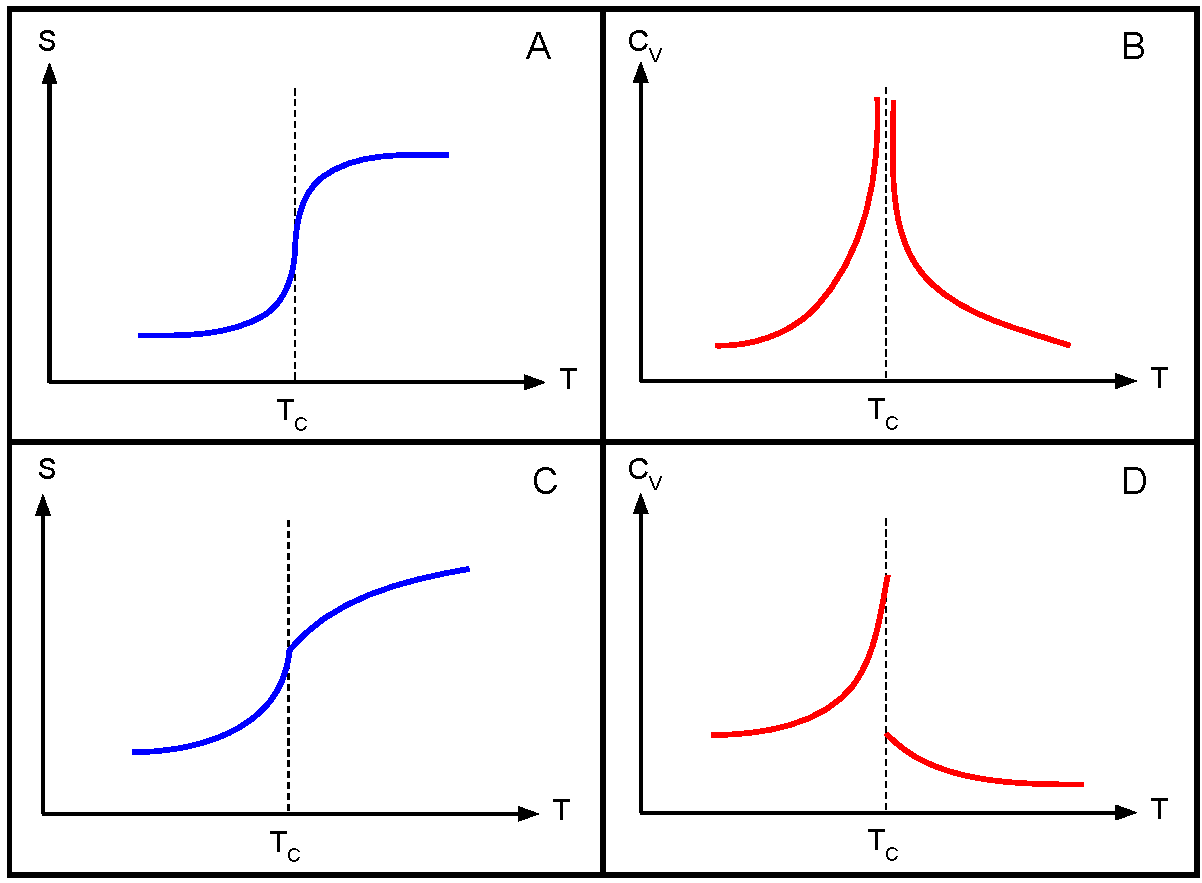
\includegraphics[width = 0.75\textwidth]{chapter2Figs/CanonicalSecondOrder.pdf}
\caption{\label{fig:Fig_4}% 
Second order transitions are characterized by discontinuities in response quantities, such as the specific heat. (a,b) In the case of a \textbf{critical} second order transition, the entropy $S$ attains an infinite slope at $T_{c}$ accompanied by a divergence in the specific heat $C_{V}$. (c,d) So called \textit{lambda} transitions are characterized by a jump discontinuity in $C_{V}$ and a cusp singularity in entropy.}
\end{figure}

Second order transitions do not posses discontinuities in entropy, and for that reason are often called \textit{continuous} transitions. Instead, discontinuities are found in the second derivatives of the free energy with respect to temperature. It is customary to make use of equation\,\,\ref{eq:22}, and consider the specific heat $C_{V}$ which also contains the same discontinuities.
In the vicinity of the transition point $T_{c}$, the specific heat exhibits a power law behavior $C_{V}(\tau) \propto \left| \tau \right|^{-\alpha}$, where $\tau = \left(T-T_{c}\right)/T_{c}$ and $\alpha$ is the associated critical exponent. Examples of common types of discontinuities of $C_{V}$ are shown in Fig. \ref{fig:Fig_4}. Other important quantities such as the magnetic susceptibility $\chi$ and the correlation length $\xi$ also exhibit a power law behavior near the transition point, governed by the critical exponents $\gamma$ and $\nu$ respectively. The striking observation, that in the vicinity of the critical temperature $T_{c}$, the behavior of physical systems with diverse microscopic properties can be described in terms of the same critical exponents, is formalized in the theory of Universality\cite{Kardar2009}. 

\subsubsection{Canonical analysis in mesoscopic systems} 
The description of phase transitions in the terms of discontinuities and divergences is valid only in the thermodynamic limit. In situations where the thermodynamic behavior of a system is affected by finite size effects, this idealized description no longer applies. Nevertheless, the numerous examples of abrupt changes of macroscopic properties in finite systems necessitate the generalization of the theory. In order to avoid possible confusion, we shall refer to significant conformational changes in finite systems as \textit{pseudophase transitions}. Similarly, sets of macrostates with sufficiently similar macroscopic properties will be denoted \textit{pseudophases}.

In the generalized formalism, peaks in the specific heat and other response quantities indicate regions of increased thermodynamic activity, i.e. pseudophase transitions. The order of the transition is determined from the shape of the canonical energy distribution in the transition region. Bimodal distributions reveal the coexistence of two pseudophases and indicate a first-order transition\cite{Janke1998}. The associated latent heat of the transition is given by the energetic separation between the two peaks in the distribution. Second-order transitions correspond to unimodal energy distributions. The power law behavior of response quantities contains significant finite-size corrections and in some cases is altogether not applicable\cite{Landau2000}. An example of canonical analysis, applied to first- and second-order pseudophase transitions, is illustrated in Fig. \ref{fig:Fig_5}. 

\begin{figure}
\center
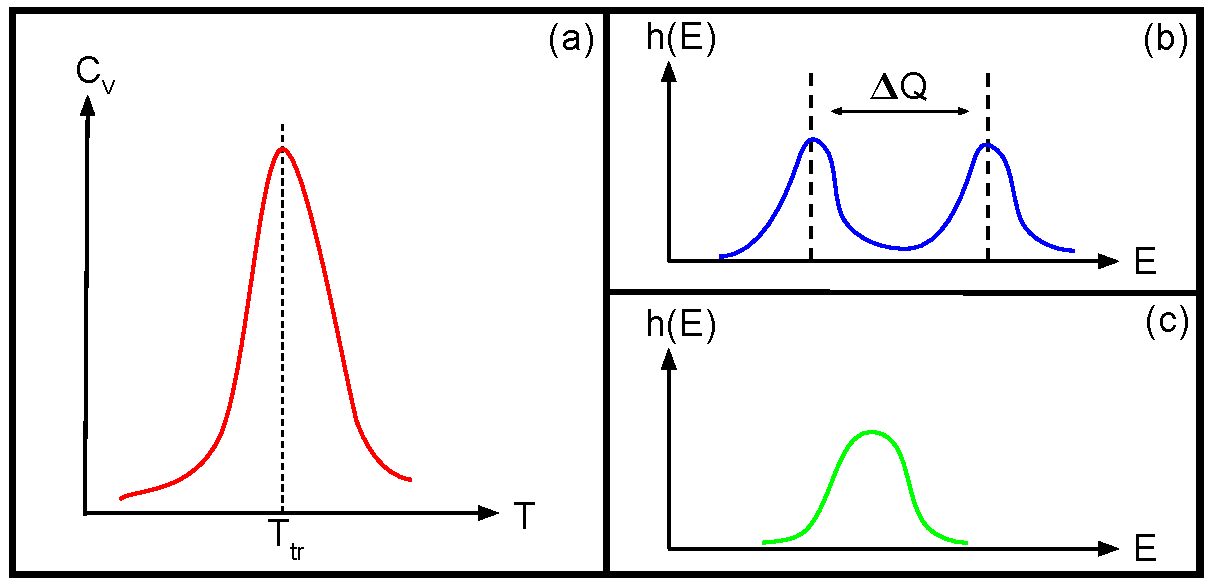
\includegraphics[width = 0.8\textwidth]{chapter2Figs/CanonicalAnalysisSample.pdf}
\caption{\label{fig:Fig_5}% 
(a) The peak in the specific heat $C_{V}$ indicates a region of heightened thermodynamic activity. (b) The two peaks in the bimodal canonical energy distribution correspond to the ordered and disordered pseudophases, energetically separated by the latent heat $\Delta Q$. Pseudophase coexistence and latent heat are reliable indicators of a first-order pseudophase transition. (c) Second-order transitions are marked by wide unimodal energy distributions at the transition point.}
\end{figure}

It should be mentioned that second-order pseudophase transitions do not always produce peaks in the specific heat. In general, it is necessary to investigate the behavior of several response quantities in order to obtain an accurate picture of the transition properties of the system under investigation. However, due to finite size effects, the signals obtained from different quantities will in general not coincide at a single transition temperature. This reality further fortifies the argument that the microcanonical inflection-point analysis\footnote{Introduced in Sec. \ref{subsec: micro_analysis}}, which defines a unique transition temperature in mesoscopic and macroscopic systems alike, is the preferred formalism for the analysis of finite systems.
\newpage

\section{Alternative definitions of the density of states}
In section \ref{sec:mic_ensemble} we have defined the microcanonical density of states $g(E)$ as an integral over the surface of constant energy in the $6N$-dimensional phase space. We have argued that $g(E)$ contains all the essential information about the thermodynamic properties of the system under consideration, and introduced the formalism of the microcanonical inflection-point analysis which uses the logarithm of $g(E)$ as its starting point. In section \ref{sec:canonicalEnsemble} we have shown that the canonical partition function $Z(T)$ can be obtained by performing a Laplace transform of $g(E)$. Clearly, the microcanonical density of states plays a fundamental role in equilibrium statistical mechanics, and as such needs to be carefully defined. 

Two distinct definitions of the density of states arise from certain ambiguity in the exact meaning of the microcanonical ensemble in computational studies. The density of states can be defined in the context of the conformational microcanonical ensemble $(N,V,E_{p})$ as a function of the potential energy only
\begin{equation}
g_{c}(E_{p}) = \int \mathcal{DQ} \:\: \delta(E_{p} - \mathcal{H}(\mathcal{Q}))
\end{equation}
This definition is commonly used in Monte Carlo simulations of magnetic systems where the kinetic energy contributions have little physical significance and the sampling can be restricted to the conformational space. However, in systems where the transfer between potential and kinetic energy has important physical interpretation, the sampling of the full phase space becomes necessary. The standard definition of the microcanonical ensemble $(N,V,E)$ is applied and the measured density of states becomes a function of the total system energy, which can be written as the sum of the potential and kinetic energies
\begin{equation}
E = E_{p} + E_{k}.
\end{equation}
In order to distinguish between the two definitions, we shall use the symbol $\Gamma(E)$ to represent the latter definition of the density of states. The connection between the conformational density of states and $\Gamma(E)$ is expressed as a convolution\cite{Calvo1995}
\begin{equation}
\label{eq:TotalDOS}
\Gamma(E) = \int dE_{k} \: g_{c}(E - E_{k})g_{k}(E_{k}),
\end{equation}
where 
\begin{equation}
g_{k}(E_{k}) = \int \mathcal{DP} \:\: \delta(E_{k} - \mathcal{H}(\mathcal{P}))
\end{equation}
is the kinetic density of states obtained by integrating over the momentum space.

We shall now turn our attention to the consequence of choosing either the conformational or the full density of states as the starting point for a systematic analysis of the thermodynamic properties of a system under consideration. In the following we will discuss the impact of ignoring the momentum degrees of freedom on the results of both the canonical and microcanonical analysis. As an illustration, we will provide results from Monte Carlo simulations of two short flexible homopolymers.

\subsection{Consequences for canonical analysis}
The canonical partition function $Z(T)$ and the microcanonical density of states are connected via a Laplace transform. We begin with the full density of states $\Gamma(E)$ and using the definition from Eq. \ref{eq:TotalDOS} write
\begin{equation}
\label{eq:Laplace}
Z(T) = \mathcal{L}\left\lbrace\Gamma(E)\right\rbrace = \mathcal{L}\{g_{c} \ast g_{k} \} = \mathcal{L}\{g_{c}\} \mathcal{L}\{g_{k}\},
\end{equation}
where the last step follows from the convolution theorem\cite{Arfken}. 
\newpage
\noindent
The partition function of the system can hence be conveniently written as a product of two independent partition functions
\begin{equation}
Z(T) = Z_{c}(T)Z_{k}(T),
\end{equation}
which depend on the potential and kinetic energies respectively. It follows that the average ensemble energy can be expressed as the sum of the average potential and kinetic energies
\begin{eqnarray}
U(T)  &=& k_{\mathrm{B}}T^{2}\frac{\partial}{\partial T} \mathrm{ln} Z\bigg|_{N,V} \nonumber \\
	 &=& k_{\mathrm{B}}T^{2}\frac{\partial}{\partial T} \mathrm{ln} Z_{c} \bigg|_{N,V}	 + k_{\mathrm{B}}T^{2}\frac{\partial}{\partial T} \mathrm{ln} Z_{k} \bigg|_{N,V}	 \nonumber \\
	 &=& \langle E_{c} \rangle + \langle E _{k}\rangle.  
\end{eqnarray}
With the exception of systems with rigid constraints, the average kinetic energy is given by the equipartition theorem 
\begin{equation}
 \langle E _{k}\rangle = \frac{3Nk_{\mathrm{B}}T}{2},
\end{equation}
where $N$ is the number of particles in the system. It follows that the specific heat $C_{\mathrm{V}}$ obtains only a trivial additive constant from the kinetic energy term
\begin{eqnarray}
C_{\mathrm{V}}(T) &=& \frac{\partial}{\partial T} U(T)\bigg|_{N,V} \nonumber \\
				 &=& \frac{\partial}{\partial T} \langle E_{c} \rangle\bigg|_{N,V} + \frac{\partial}{\partial T}\frac{3Nk_{\mathrm{B}}T}{2} \nonumber \\
				 &=& C_{\mathrm{V},\mathrm{conf.}} + \frac{3Nk_{\mathrm{B}}}{2}.
\end{eqnarray}

\begin{figure}
\center
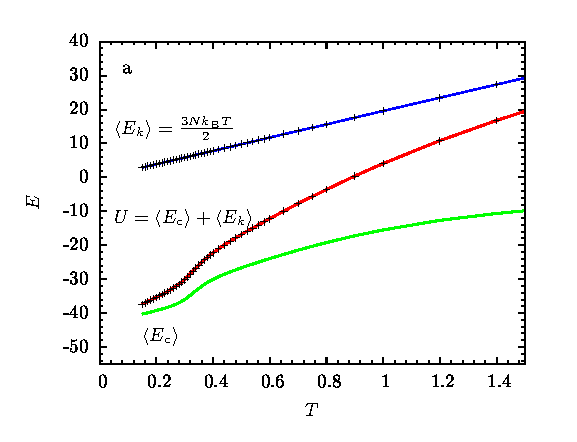
\includegraphics[width = 0.49\textwidth]{chapter2Figs/N13Energy.eps}
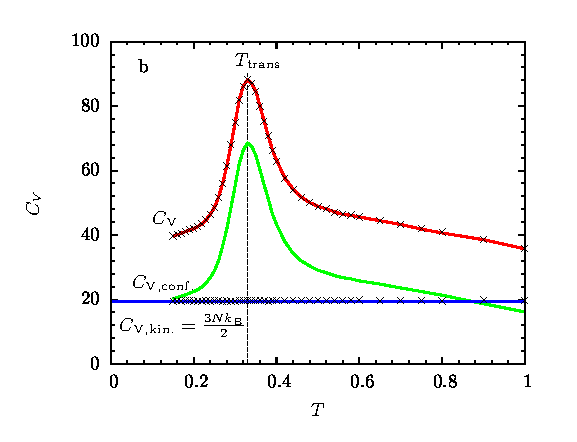
\includegraphics[width = 0.49\textwidth]{chapter2Figs/N13Spec.eps}
\caption{\label{fig:Fig_6}% 
Results of a Monte Carlo simulation of a short flexible homopolymer of length $N=13$. The average kinetic energy $\langle E _{k}\rangle$ and the kinetic contributions $C_{\mathrm{V,kin.}}$ towards the specific heat are plotted as points on top of their respective theoretical curves (blue). The average potential energy $\langle E_{c} \rangle$ and the configurational specific heat $C_{\mathrm{V},\mathrm{conf.}}$ (green) were obtained by sampling of the configurational space. Sampling of the full phase space was performed to obtain the total average energy $U$ and the combined specific heat $C_{\mathrm{V}}$ (red). As expected, the combined specific heat is identical to $C_{\mathrm{V},\mathrm{conf.}}$, except for a trivial additive constant.}
\end{figure}

In conclusion, the locations and shapes of signals for pseudophase transitions are not affected by the inclusion of the momentum space into a sampling scheme. To substantiate this assertion, in Fig. \ref{fig:Fig_6} we present the results from a Monte Carlo study of a short flexible homopolymer. The average kinetic energy $\langle E _{k}\rangle$ and the kinetic contributions $C_{\mathrm{V,kin.}}$ towards the specific heat are plotted as points on top of their respective theoretical curves (blue), showing good agreement with the predicted values. The average potential energy $\langle E_{c} \rangle$ and the configurational specific heat $C_{\mathrm{V},\mathrm{conf.}}$ (green) were obtained by the sampling of the configurational space only. Sampling of the full phase space was performed to obtain the total average energy $U$ and the combined specific heat $C_{\mathrm{V}}$ (red). As expected, the combined specific heat is identical to $C_{\mathrm{V},\mathrm{conf.}}$, except for a trivial additive constant. The estimate of the transition temperature is independent of the choice of either definition of the density of states. 
\newpage 

\subsection{Consequences for microcanonical analysis}
The application of the Laplace transform to the total density of states $\Gamma (E)$, allowed us to conveniently disentangle the convolution in Eq.\,\,\ref{eq:TotalDOS} \, into separate kinetic and conformational contributions [Eq. \ref{eq:Laplace}]. Unfortunately, in the microcanonical ensemble no such simplification is readily available. Let us however consider a class of physical systems whose momenta and positional degrees of freedom are independent. Explicit integration over the momentum space yields a simple expression for the kinetic density of states
\begin{equation}
g_{k}(E_{k}) = \int \mathcal{DP} \:\: \delta(E_{k} - \mathcal{H}(\mathcal{P})) 
			 = E_{k}^{\frac{3N-2}{2}}.
\end{equation}
Combining the result with Eq. \ref{eq:TotalDOS} \, we obtain
\begin{equation}
\Gamma(E) = \int dE_{k} \: g_{c}(E - E_{k})E_{k}^{\frac{3N-2}{2}}.
\end{equation}
Next, taking a derivative with respect to the total energy $E$ and dividing both sides by $\Gamma(E)$ we get two equivalent expressions for the microcanonical inverse temperature 
\begin{eqnarray}
\beta(E) &=& \int dE_{k} \:\frac{3N-2}{2E_{k}} \:\left[\frac{g_{c}(E - E_{k})E_{k}^{\frac{3N-2}{2}}}{\Gamma (E)}\right]
\label{eq:beta1}  \\
		&=& \int dE_{p} \: \beta_{c}(E_{p})\: \left[ \frac{g_{c}(E_{p})(E- E_{p})^{\frac{3N-2}{2}}}{\Gamma (E)} \right]
\label{eq:beta2}.  
\end{eqnarray}
Recognizing the two terms enclosed in square brackets as the microcanonical probability densities for the kinetic and potential energies,
we can rewrite equations \ref{eq:beta1} and \ref{eq:beta2} as
\newpage
\noindent
\begin{equation}
\label{eq:beta3}
\beta(E) = \int dE_{k} \:\frac{3N-2}{2E_{k}} \: \rho(E_{k})_{E} = \frac{3N-2}{2}\left\langle \frac{1}{E_{k}}  \right\rangle,
\end{equation}
and 
\begin{equation}
\label{eq:beta4}
\beta(E) = \int dE_{p} \: \beta_{c}(E_{p})\: \rho(E_{p})_{E} = \left\langle \beta_{c} \right\rangle.
\end{equation}
The microcanonical inverse temperature, obtained by the differentiation of the total density of states, can therefore be interpreted as an average of the conformational and kinetic anologs weighted by their respective microcanonical probability distributions.

When the number of particles in the system is large, the probability densities $\rho(E_{k})_{E}$ and $\rho(E_{p})_{E}$ are expected to be sharply peaked around the most probable kinetic $\bar{E}_{k}$ and potential $\bar{E}_{p}$ energies respectively . We can therefore apply the saddle point approximation to the integrals in equations [\ref{eq:beta3}, \ref{eq:beta4}] and obtain the following first order approximations for the inverse temperature
\begin{equation}
\label{eq:approx1}
\beta(E) \approx \beta_{c}(\bar{E}_{p}),
\end{equation}
and
\begin{equation}
\label{eq:approx2}
\beta(E) \approx \frac{3N-2}{2}\left(\frac{1}{\bar{E}_{k}}\right). 
\end{equation}
The first expression suggests that it is possible to reconstruct $\beta(E)$ from the conformational inverse temperature $\beta_{c}$, and that the two quantities contain essentially the same information. We test the validity of this hypothesis by comparing the microcanonical results of Monte Carlo simulations of a flexible elastic $55-$mer, which were carried out in both the conformational space and the full phase space.
\newpage
\begin{figure}
\center
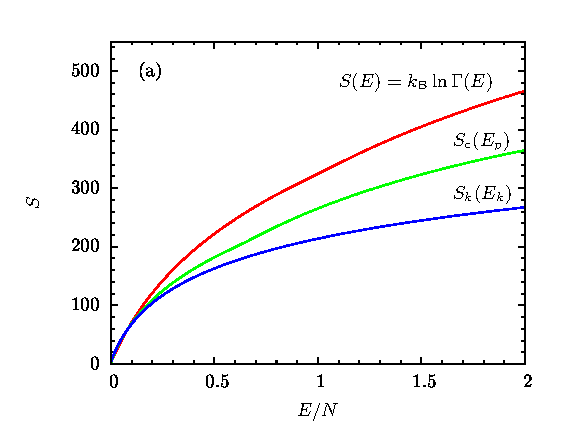
\includegraphics[width = 0.49\textwidth]{chapter2Figs/N55Entropy.eps}
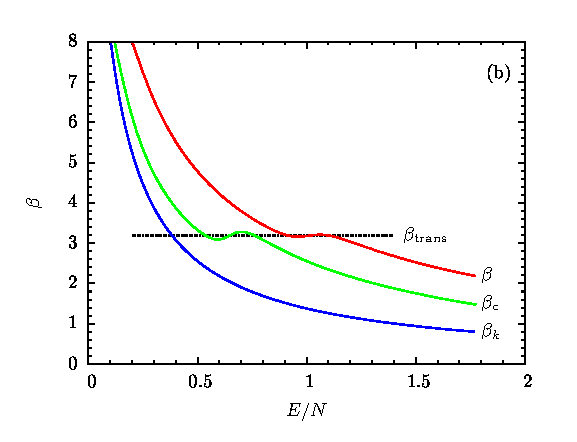
\includegraphics[width = 0.49\textwidth]{chapter2Figs/N55Beta.eps}
\caption{\label{fig:Fig_7}% 
Comparison of microcanonical results from a Monte Carlo simulation of a flexible homopolymer of length $N=55$.(a) The combined $S$, conformational $S_{c}$, and kinetic $S_{k}$ entropy curves. (b) The kinetic inverse temperature $\beta_{k}$ is a strictly convex function and the application of the inflection-point analysis reveals no transition signals. The conformational inverse temperature $\beta_{c}$ clearly differs from $\beta(E)$, however both indicate a first-order pseudophase transition at virtually the same temperature. }
\end{figure}
The kinetic entropy in Fig. \ref{fig:Fig_7} is a strictly concave function and the application of the inflection-point analysis to the corresponding inverse temperature $\beta_{k}$ reveals no transition signals. The conformational inverse temperature clearly differs from $\beta(E)$, however both indicate a first-order pseudophase transition at virtually the same temperature. In Fig. \ref{fig:Fig_8} we show the comparison between the true $\beta(E)$ and the reconstruction obtained from the conformational inverse temperature according to equations \ref{eq:approx1} and \ref{eq:approx2}. It is evident that the approximation is valid, except in the back-bending region of the first-order transition due to the bimodality of the probability densities $\rho(E_{k})_{E}$ and $\rho(E_{p})_{E}$. 

\newpage
The expression in equation \ref{eq:approx2} can be rewritten as 
\begin{equation}
k_{\mathrm{B}}T(E) \approx \frac{2}{3N-2}\left(\frac{1}{\bar{E}_{k}}\right)^{-1},
\end{equation}
which clearly resembles the well known relationship between the canonical temperature and the average kinetic energy. In the the thermodynamic limit, this approximation becomes exact and the equivalency of the microcanonical and canonical ensembles is restored. 



\begin{figure}
\center
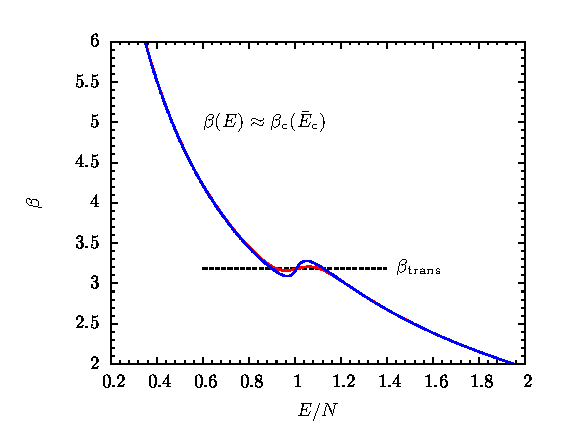
\includegraphics[width = 0.7\textwidth]{chapter2Figs/N55BetaComp.eps}
\caption{\label{fig:Fig_8}% 
Comparison of the inverse microcanonical temperature $\beta(E)$ (red) and the conformational inverse temperature $\beta_{c}(\bar{E}_{p})$ (blue) evaluated at the most probable potential energy $\bar{E}_{p}$. The approximation introduced in equation \ref{eq:approx1} holds except in the back-bending region of the first-order pseudophase transition. The inverse transition temperature $\beta_{\mathrm{trans}}$ obtained from the two quantities is virtually identical.}
\end{figure}

%%%%%%%%%%%%%%%%%%%%%%%%%%%%%%%%%%%%%%%%%%%%%%%%%%%%%%%%%%%%%%%%%%%%%%%%%%%%%%%%%%%%
%%%%%%%%%%%%%%%%%% 			CHAPTER 3     		%%%%%%%%%%%%%%%%%%%%%%%%%%%%%%%%%%%
%%%%%%%%%%%%%%%%%%%%%%%%%%%%%%%%%%%%%%%%%%%%%%%%%%%%%%%%%%%%%%%%%%%%%%%%%%%%%%%%%%%%

\chapter{Computational Methods}

Computational algorithms are powerful tools that enable the investigation of physical systems that are far too complex to be solved analytically.
In fact, only a handful of systems are exactly solvable\footnote{The most prominent examples are the ideal gas and the two dimensional Ising model.} and even the simplest solutions require bewildering mathematical gymnastics. Consequently, computational studies are the main source of advances in the fundemental understanding of complex microscopic and mesoscopic systems such as biopolymers and proteins.

Two complementary classes of computational algorithms have been particularly successful in unravelling the thermodynamic properties of physical systems. \textit{Molecular dynamics} simulations generate a single phase space trajectory by updating the positions and momenta of every particle in a system according to Hamilton's equations. On the other hand, carrying out a stochastic sampling of the phase space, \textit{Monte Carlo} simulations estimate the equilibrium properties without the explicit consideration for the system's dynamics. In this chapter, we shall focus our attention to Markov chain Monte Carlo methods. We will briefly discuss the essential theory and introduce the well established Metropolis and Parallel Tempering algorithms as well as the lesser known Multiple Gaussian modified ensemble method.



\section{Markov chain Monte Carlo}
The aim of all Monte Carlo methods is to extract the equilibrium thermodynamic properties of physical systems by performing an efficient stochastic sampling of the phase space. For this purpose, a set of random microstates $\{\mu_{1},\mu_{2},...,\mu_{M}\}$ is generated according to some previously known probability distribution $p(\mu_{i})$, and the expectation value for any observable $O({\mu})$ is estimated by calculating the average
%
\begin{equation}
\label{eq:expectationValue}
\bar{O} = \frac{1}{M}\sum_{i = 1}^{M} O(\mu_{i}).
\end{equation}
%
In most Monte Carlo methods, the set of random microstates is generated according to a discrete-time Markov chain (DTMC). Markov chains are sequences of random states, generated according to the time-independent transition probabilities 
$T(\mu \rightarrow \nu)$ which satisfy the Markov property. In simple terms, the probability of moving to state $\nu$ from state $\mu$ depends only on the present state, and is independent of the history of the process. In order to achieve the correct statistical sampling of an equilibrium thermodynamic ensemble, the following conditions must also be satisfied.

The process must be \textbf{ergodic}, i.e., there must be a path of non-zero probability between any pair of states. More formally, the state space $\mathcal{S}$ of the Markov chain must consist of a single aperiodic recurrence class. When ergodicity is satisfied, the ensemble average $\left\langle O \right\rangle$ can be approximated by the measured expectation value $\bar{O}$ [Eq. \ref{eq:expectationValue}] 
%
\begin{equation}
\label{eq:approximationOfExpectationValues}
\bar{O} = \frac{1}{M}\sum_{i = 1}^{M} O(\mu_{i}) \approx \left\langle O \right\rangle = \int \mathcal{DP}\mathcal{DQ} \:\: O(\mathcal{P},\mathcal{Q})
p(\mathcal{P},\mathcal{Q}),
\end{equation}
%
where $M$ is the length of the Markov chain. According to the ergodic hypothesis, the approximation becomes exact in the limit of an infinitely long Markov chain
%
\begin{equation}
\label{eq:ergodicHyp}
\lim_{M\rightarrow \infty}\frac{1}{M}\sum_{i = 1}^{M} O(\mu_{i}) = \int \mathcal{DP}\mathcal{DQ} \:\: O(\mathcal{P},\mathcal{Q})
p(\mathcal{P},\mathcal{Q}).
\end{equation}
%
%
The time evolution of a discrete-time Markov process is described by the master equation
%
\begin{equation}
\label{eq:MasterEquation}
\frac{\Delta p(\mu)}{\Delta t} = \sum_{\nu} p(\nu)T\left(\nu \rightarrow \mu\right) - p(\mu)T\left(\mu \rightarrow \nu\right).
\end{equation}
%
The equilibrium condition requires that the probability distribution $p(\mu)$ is stationary. In other words, the probability currents into and out of the state $\mu$ must be always equal
\begin{equation}
\label{eq:balance}
\sum_{\nu} p(\nu)T\left(\nu \rightarrow \mu\right) = \sum_{\nu} p(\mu)T\left(\mu \rightarrow \nu\right).
\end{equation}
%
Also known as the $\textbf{balance}$ condition, equation \ref{eq:balance} sometimes allows for solutions that are not permitted in the equilibrium ensemble. The stricter condition of $\textbf{detailed balance}$ requires that the probability of a transfer between any two states must be equal to the probability of the reverse process. Embodied in the expression
%
\begin{equation}
\label{eq:detailedBalance}
p(\mu)T\left(\mu \rightarrow \nu\right) = p(\nu)T\left(\nu \rightarrow \mu\right),
\end{equation} 
%
this condition is sufficient to prevent any non-physical solutions as well as to ensure that the process is invariant under time reversal.


Having introduced the conditions of ergodicity and detailed balance, we can now derive the expression for transition probabilities which will ensure correct stochastic sampling according to an equilibrium distribution $p\left(\mu\right)$. 
For convenience, we will separate the transition probabilities into two separate terms and write


%
\begin{equation}
\label{eq:factoredTransitionProb}
T\left(\mu \rightarrow \nu\right) = s\left(\mu \rightarrow \nu\right)a\left(\mu \rightarrow \nu\right).
\end{equation}
Assuming the current state $\mu$, the probability of generating a new state $\nu$ is given by the selection probability $s\left(\mu \rightarrow \nu\right)$, while the probability of accepting the proposed update is controlled by the \textit{acceptance} probability $a\left(\mu \rightarrow \nu\right)$. Combining equations \ref{eq:detailedBalance} and \ref{eq:factoredTransitionProb}, we express the ratio of the transition probabilities as
%
\begin{equation}
\label{eq:ratioOfTransitionProb}
\frac{T\left(\mu \rightarrow \nu\right)}{T\left(\nu \rightarrow \mu\right)} = \frac{s\left(\mu \rightarrow \nu\right)a\left(\mu \rightarrow \nu\right)}{s\left(\nu \rightarrow \mu\right)a\left(\nu \rightarrow \mu\right)} = \frac{p\left(\nu\right)}{p\left(\mu\right)}.
\end{equation}
%
The ratio of the forward and backward selection probabilities
$\sigma(\mu,\nu) = s\left(\mu \rightarrow \nu\right)/s\left(\nu \rightarrow \mu\right)$
depends on the choice of the particular update scheme. In the remainder of this thesis, we shall assume that the forward and backward selection probabilities are equal and the ratio equals to unity, which is valid for most local Monte Carlo updates. This simplifying assumption allows us to rewrite equation \ref{eq:ratioOfTransitionProb} without making explicit references to the selection probabilities
%
\begin{equation}
\label{eq:acceptanceProbs}
\frac{a\left(\mu \rightarrow \nu\right)}{a\left(\nu \rightarrow \mu\right)} = \frac{p\left(\nu\right)}{p\left(\mu\right)}.
\end{equation}
%

\subsection{Metropolis sampling}

Any set of acceptance probabilities which satisfies equation \ref{eq:acceptanceProbs} is allowable, however the standard choice is to set the higher of the two probabilities to unity. This yields the well known Metropolis acceptance criterion:
%
\begin{equation}
\label{eq:MetropolisCriterion}
a\left(\mu \rightarrow \nu\right) = \mathrm{min}\left(1,\frac{p\left(\nu\right)}{p\left(\mu\right)} \right).
\end{equation}
% 
Under most circumstances, Metropolis sampling is carried out according to the canonical microstate probability distribution $p(\mu) \propto e^{-\beta E(\mu)}$, where $\beta$ is the inverse canonical temperature. Hence the acceptance probability is governed by the energy difference between the proposed and the current states
%
\begin{equation}
\label{eq:MetropolisCriterionCanonical}
a\left(\mu \rightarrow \nu\right) = \mathrm{min}\left(1,\frac{e^{-\beta E(\nu)}}{e^{-\beta E(\mu)}} \right) = \mathrm{min}\left(1,e^{-\beta \Delta E} \right).
\end{equation}
%
The average of the observable $O(\mu)$, measured over the length of a finite Metropolis run, serves as an estimate for the canonical expectation value $\left\langle O \right\rangle$ [Eq.\,\,\ref{eq:approximationOfExpectationValues}]. 
In the limit of an infinite run, this approximation becomes exact [Eq.\,\,\ref{eq:ergodicHyp}]. However, since all simulations are of finite length, it is imperative to account for the statistical errors introduced due to the finiteness of the measured data sets. The standard bias corrected error estimator for the calculated average $\bar{O}$, obtained from a finite set of $M$ uncorrelated measurements, is written as
%
\begin{equation}
\mathrm{err}(\bar{O}) = \pm \,\,\sqrt{\frac{1}{M(M-1)} \sum_{m} (O_{m} - \bar{O})^{2}}.
\end{equation}
%
In reality, most measurements obtained from Monte Carlo simulations are correlated. Hence it is necessary to introduce the modified error estimator
%
\begin{equation}
\mathrm{err}(\bar{O}) = \pm \,\,\sqrt{\frac{1}{M(M_{\mathrm{eff}}-1)} \sum_{m} (O_{m} - \bar{O})^{2}},
\end{equation}
%
where $M_{\mathrm{eff}}$ is the number of uncorrelated measurements\footnote{For detailed description of the more practical \textit{binning} and \textit{jackknife} error estimation methods, please refer to chapter 4 in \cite{Bachmann2014}.}.

The Metropolis method provides the means for an efficient sampling of microstates which are dominant at a given temperature. However, the microstates which are found in the tails of the canonical energy distribution are rarely visited. Further shortcomings of the Metropolis algorithm, such as the propensity for getting trapped in low-energy configurations and the notorious reduction in sampling efficiency near pseudophase transitions, motivate the introduction of more efficient sampling methods.


\subsection{Parallel tempering}
In situations where the Metropolis method fails to produce data of reasonable quality, the standard way of increasing sampling efficiency is to perform the simulation in a conveniently chosen \textit{generalized ensemble}\footnote{The microstate probability distribution of a generalized ensemble can be arbitrary and does not have to bear any resemblance to the Boltzmann distribution.}. In parallel tempering, multiple canonical ensembles with different inverse temperatures $\{\beta_{1} < \beta_{2} < ... < \beta_{N}\}$ are simulated in parallel according to the standard Metropolis scheme. In this context, the generalized ensemble is defined as the direct product of $N$ canonical ensembles, and the partition function is given by
%
\begin{equation}
Z_{\mathrm{PT}}(\beta_{1},\beta_{2},...,\beta_{N}) = \prod_{i=1}^{N} Z_{\mathrm{can}}(\beta_{i}).
\end{equation}
%
At judiciously chosen intervals, an exchange of conformations between adjacent temperature threads $i$ and $j$ is proposed. The combined probability for states $(\mu, \, \nu)$ at respective temperatures $(\beta_{i}, \, \beta_{j})$ is given by
\begin{equation}
p_{\mu\nu} =  \frac{\displaystyle e^{-\beta_{i}E(\mu)}}{\displaystyle Z_{\mathrm{can}}(\beta_{i})} \frac{\displaystyle e^{-\beta_{j}E(\nu)}}{\displaystyle Z_{\mathrm{can}}(\beta_{j})},
\end{equation}
%
and the acceptance probability for the exchange of conformations is obtained from Eq. \ref{eq:MetropolisCriterion}
%
\begin{eqnarray}
\label{eq:replicaExchange}
a\left(\mu \leftrightarrow \nu;\beta _{i}, \beta_{j} \right) &=&
\mathrm{min}\left(1, \frac{\displaystyle e^{-\beta_{i}E(\nu)}e^{-\beta_{j}E(\mu)}}{\displaystyle e^{-\beta_{i}E(\mu)}e^{-\beta_{j}E(\nu)}}\right) \nonumber \\
&=&
\mathrm{min}\left(1,e^{\left[\beta_{j} -
\beta _{i} \right] \left[E (\nu) -
E(\mu)\right]} \right).
\end{eqnarray}
%
The exchange rates are governed by the overlap of canonical energy distributions of the adjacent ensembles, hence the efficiency of the method depends sensitively on the choice of an appropriate temperature set. As a general rule, the density of temperatures must be increased in ordered phases and in the vicinity of pseudophase transitions. 

In principle, each replica is allowed to traverse the entire simulated
temperature range which leads to the decrease of the autocorrelation time and reduces the likelihood of getting trapped in local energy minima at low temperatures. However, the performance of this method rapidly decreases near first-order transitions, where the joint effects of the entropic suppression of intermediate states and the energetic separation between the ordered and disordered pseudophases, virtually prevent the exchange of configurations between adjacent ensembles.
 
\subsection{Multiple Gaussian modified ensemble}

An alternative generalized ensemble method that offers improved performance is based on the combination of parallel tempering with the Gaussian modified ensemble (GME) method. The idea behind GME is to modify the canonical Boltzmann distribution by multiplying it by a Gaussian function, in order to promote sampling in selected energy regions. The mean energy $E_{G}$ and the variance $\Delta E_{G}^{2}$ of the Gaussian form controls the location and the width of the region of enhanced sampling. The modified microstate probability at the inverse temperature $\beta$ is given by
%
\begin{equation}
P_{\mathrm{GME}}(\mu) \propto e^{-\beta E_{\mu} -
\left(E_{\mu} - E_{G}\right)^{2} / \Delta E_{G}^{2}}.
\end{equation}
% 
The measurements obtained from simulations in a modified ensemble must be reweighted in order to obtain the expectation values in the original canonical ensemble. In the context of the modified Gaussian ensemble this is done by calculating
\begin{equation}
\left\langle O \right\rangle_{\mathrm{can},\beta} = \frac{\displaystyle \sum_{i=1}^{M} O_{i}e^{\beta 
\left(E_{i} - E_{G}\right)^{2} / \Delta E_{G}^{2}}}{\displaystyle \sum_{i=1}^{M} e^{\beta 
\left(E_{i} - E_{G}\right)^{2} / \Delta E_{G}^{2}}}.
\end{equation} 
%
\begin{figure}
\center
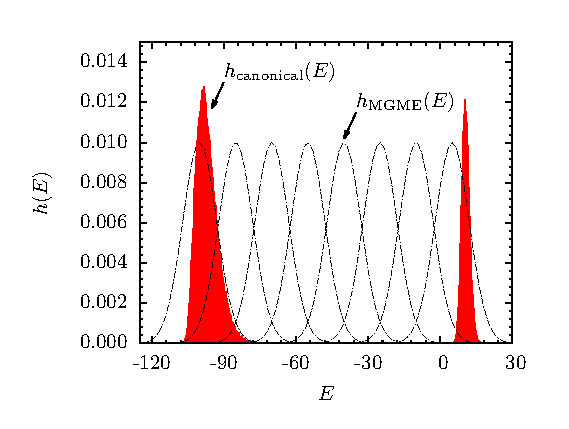
\includegraphics[width = 0.7\textwidth]{chapter3Figs/mgme.eps}
\caption{\label{fig:MGME}%
Canonical and GME energy histograms at a first-order pseudophase transition. The bimodal canonical energy histogram indicates the coexistence of ordered and disordered pseudophases, separated by an entropically suppressed energy region. Each GME ensemble enhances the sampling of suppressed states over a limited energy range.}
\end{figure} 
% 


Strong first-order transitions with bimodal energy distributions typically
require several overlapping GME ensembles to cover the relevant energy range, as illustrated in Fig.~\ref{fig:MGME}. The acceptance probability for the
exchange of conformations $(\mu,\nu)$ between neighboring GME ensembles with mean energies $(E_{G,i}, E_{G,j})$ at a constant inverse temperature $\beta$ is
%
\begin{equation}
a\left(\mu \leftrightarrow \nu \right) = 	
\mathrm{min}\left(1,e^{\Delta G}\right),
\end{equation}
%
where
\begin{equation}
\Delta G  = 
\frac{\left(E_{\mu} - E_{G,j}\right)^{2}-\left(E_{\nu}-
E_{G,j}\right)^{2}}{\Delta E_{G,j}^{2}} - \frac{\left(E_{\nu} - 	
E_{G,i}\right)^{2}-\left(E_{\mu} - E_{G,i}\right)^{2}}{\Delta E_{G,i}^{2}}.
\end{equation}

The direct product of GME ensembles defines the multiple Gaussian modified ensemble (MGME). With a proper choice of ensemble parameters $(E_{G},\Delta E_{G})$ it is possible to achieve a significantly enhanced sampling of previously inaccessible states. This can be further improved by allowing for exchanges between GME ensembles at different temperatures. However, previous knowledge of the system under consideration is usually needed to make a reasonable estimate for the ensemble parameters. Therefore other more systematic methods, such as multicanonical and Wang-Landau sampling, are often used.    


\section{Histogram reweighting methods}

In chapter \ref{chap:elements_of_stat_mech}, we have introduced the microcanonical inflection point analysis as the means for the systematic study of pseudophase transitions in the microcanonical ensemble. Application of this method however presumes the precise knowledge of the microcanonical density of states $g(E)$ [Eq \ref{eq:densitOfStatesExplicit}]. Previously introduced sampling methods do not directly measure $g(E)$ but rather generate canonical energy histograms $h(E,\beta_{i})$. Hence, it is necessary to introduce a general method for estimating the density of states from energy histograms.

\subsection{Multiple\,-histogram reweighting}
Canonical histogram $h(E,\beta_{i})$ provides an approximation for the Boltzmann distribution $p_{\mathrm{can}}(E, \beta_{i})$, which is itself proportional to the microcanonical density of states
%
\begin{equation}
\label{eq:canonicalDistribution}
h(E,\beta_{i}) \approx p_{\mathrm{can}}(E, \beta_{i}) \propto g(E)e^{-\beta_{i}E}
\end{equation}
%
Therefore each histogram yields an estimate of the density of states 
%
\begin{equation}
\label{eq:singleHistogramReweighting}
\bar{g}_{i}(E) = h(E,\beta_{i})e^{\beta _{i} E}
\end{equation}
%
%
\begin{figure}
\center
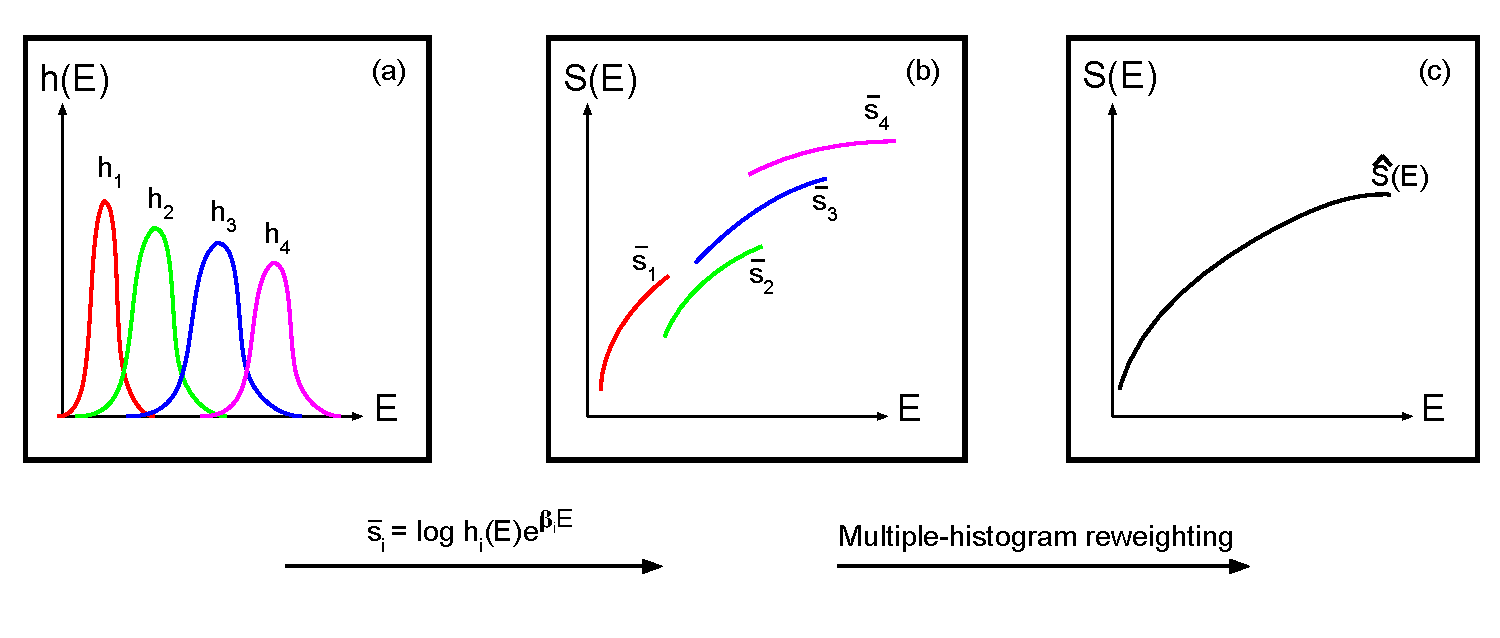
\includegraphics[width = 0.95\textwidth]{chapter3Figs/multipleHistogramReweighting.pdf}
\caption{\label{fig:MHR}%
(a) Sketch of the canonical energy histograms $h(E,\beta_{i})$, (b) the individual estimates of the logarithm of the density of states $\bar{S}_{i}(E)$, (c) and the combined estimate of the logarithm of the density of states $\hat{S}(E)$.}
\end{figure}
% 
Individual estimates $\bar{g}_{i}(E)$ are only reliable for energies in the
vicinity of the peak of the canonical histogram obtained at the temperature
$\beta _{i}$. Therefore a sufficient overlap between the histograms of
adjacent replicas is necessary to ensure that an accurate estimate of the density of states can be obtained for the entire energetic range. 

The task is now to combine the individual estimates $\bar{g}_{i}(E)$ and obtain an improved estimate $\hat{g}(E)$. Unfortunately, general Monte Carlo methods do not yield absolute estimates for the partition function $Z(\beta)$ and the estimates $\bar{g}_{i}(E)$ cannot be directly related if obtained at different temperatures.
However, it is possible to introduce a reference partition function
%
\begin{equation}
\label{eq:referencePartitionFunction}
\hat{Z}_i = \sum_E \hat{g}(E) e^{-\beta_i E},
\end{equation}
%
which serves as the appropriate weight in the estimator for the density of states
\begin{equation}
\label{eq:dosEstimator}
\hat{g}(E)= \frac{\sum_{i=1}^{R} h(E,\beta _{i})}{\sum_{i=1}^{R} M_i
\hat{Z}_i^{-1} e^{-\beta_i E}}.
\end{equation}
%
The equations \ref{eq:referencePartitionFunction} and \ref{eq:dosEstimator} must be solved iteratively until $\hat{g}(E)$ has converged. The relationship between the energy histograms, the individual estimates $\bar{g}_{i}(E)$, and the final estimate $\hat{g}(E)$ of the density of states is illustrated in Fig. \ref{fig:MHR}. For  detailed derivation and a further discussion of the multiple-histogram reweighting method please refer to \cite{Ferrenberg1989,Kumar1992}.




\subsection{Beziere smoothing}
\section{Simple Monte Carlo updates}
Mention that a proper choice of updates is equally important as choosing the right algorithm.
\subsection{Single displacement update}
Include optimization for the size of the displacement box
\subsection{Pivot update}





\chapter{Coarse-grained Homopolymer Model}
\section{Flexible elastic homopolymer}
\section{Interacting homopolymers}

\chapter{Confinement Effects on Structural Transitions in Flexible Homopolymers}
\section{Introduction}
\section{Canonical analysis}
\section{Inflection-point analysis}
\section{Hyper-phase diagrams}

\chapter{Impact of Bonded Interactions on the Ground-State Geometries of Flexible Homopolymers}
\section{Structural order parameters}
\section{15-mer}
\section{55-mer}

\chapter{Aggregation of Flexible Elastic Homopolymers}
\section{Introduction}
\section{Microcanonical analysis}
\subsection{Subphases and subphase transitions}
\subsection{Missing subphases and translational entropy}
\subsection{Density effects on the latent heat}

\chapter{Summary and Outlook}










\begin{figure}
\centerline{[ You could put a picture here. ]}
\caption{Example of a figure.}
\end{figure}

\begin{table}
\caption{Example of a table.}
\centerline{[The contents of the table would go here.]}
\end{table}



%~~~~~~~~~~~~~~~~ Reference ~~~~~~~~~~~~~~~~~~%
\addcontentsline{toc}{chapter}{Bibliography}
\begin{thebibliography}{99}
        %%%%%%%%%%% CHAPTER 2 %%%%%%%%%%%%%%%%%%
\bibitem{Bachmann2014}
M.~Bachmann, \emph{Thermodynamics and Statistical Mechanics of
Macromolecular Systems}, (Cambridge University Press, Cambridge,
2014).
%
\bibitem{Rugh2001}
H.~H.~Rugh , Phys.\ Rev.~E \textbf{64},
055101 (2001).

%%%%%%%%%%% Microcanonical Ensemble %%%%%%%%%%%

\bibitem{Kardar2007}
M.~Kardar, \emph{Statistical Physics of Particles}, (Cambridge University Press, New York, 2007).
%
\bibitem{Pathria}
R.~K.~Pathria, and P.~D.~Beale, \emph{Statistical Mechanics}, (Elsevier, Oxford, 2011).
%
\bibitem{Sethna2006}
J.~P.~Sethna, \emph{Statistical Mechanics: Entropy, Order Parameters, and Complexity}, 
(Oxford University Press, New York, 2006).
%


%%%%%%%%%%% Microcanonical Analysis %%%%%%%%%%%%
\bibitem{Gross2001} 
D.~H.~E.~Gross, \emph{Microcanonical Thermodynamics}, (World Scientific, Singapore,  2001).
%
\bibitem{Stevenson}
P.~M.~Stevenson, Phys.\ Rev.~D \textbf{23}, 2916 (1981).
%
\bibitem{Schnabel2011}
S.~Schnabel, D.~T.\ Seaton, D.~P.\ Landau, and M.~Bachmann, Phys.\ Rev.~E
\textbf{84}, 011127 (2011). 
%


%%%%%%%%%%% Canonical Analysis %%%%%%%%%%%%%%%%

\bibitem{Landau2000}
D.~P.\ Landau, and K.~Binder, \emph{A Guide to Monte Carlo Simulations in Statistical Physics}, (Cambridge University Press, Cambridge, 2000).

%%%%%%%%%%% Definitions of Density of States %%%%%%%%%

\bibitem{Calvo1995}
F.~Calvo, and P.~Labastie,  Chem.\ Phys.\ Lett. \textbf{247}, 395 (1995).
%




\end{thebibliography}


\end{document}


